\section{Creating Particular Models with Mechanical Energies}
\label{act2.1.3}

\begin{overview}

\noindent\textbf{Overview:} The problems in this section illustrate how we can use the \EnergyInteractionModel{} to answer questions and make predictions about the allowed behavior of interacting objects that are difficult to approach in any other way.
	
\end{overview}


\subsection{Three Thrown Rocks}
\label{act2.1.3a}

\begin{fnt}
	Before we start with this problem, let's review what the \EnergyInteractionModel{} does for us. As we have said before, conservation of energy relates values of certain physical parameters at the beginning of a process to the values of those parameters at the end of the process. The parameters are typically the indicators of the energy systems that change during the process or interaction. If we have a question about -- or want to predict values for -- some parameter and this parameter happens to be an indicator of an energy system, or a coefficient in an expression for an energy system, then we can proceed to construct a particular model and see if it gets us what we want.\\

\begin{wrapfigure}{R}{.2\textwidth}
	\centering
	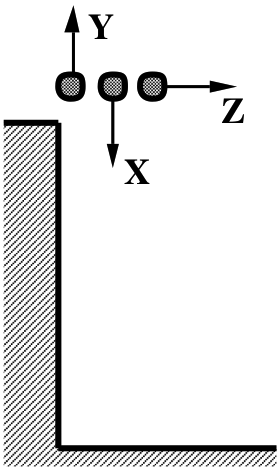
\includegraphics[width=.98\linewidth]{fnt211-rocksxyz}	
\end{wrapfigure}

\label{fnt2.1.1-1}

\noindent\textbf{The Phenomena}: Three rocks of equal mass are thrown with identical speeds from the top of the same building. (1) Rock X is thrown vertically downward, (2) Rock Y is thrown vertically upward, and (3) Rock Z is thrown horizontally.\\

\noindent\textbf{The Question}: Which rock has the greatest speed just before it hits the ground? Assume air resistance is negligible.\\

\noindent How can we determine this? We could take a guess, but it helps our argument if it is possible to apply the \EnergyInteractionModel{}. The prompts below will guide you through the process.

\begin{enumerate}[(a)]
	\item Let's start by making a prediction based on your prior experience. Don't waste a lot of time on this right now, but it's useful to give it some thought. We will definitely come back to this at the end in \hyperref[fnt211-1f]{Part~(\ref*{fnt211-1f})}. Your first, intuitive ideas might be very useful!
	\label{fnt211-1a}
	
	\item Does the question involve a parameter that you know to be an indicator of the change in an energy system? Which energy system and what is the indicator?
	\label{fnt211-1b}
	
	\item \textbf{Rock X}: Construct an \EnergyDiagram{} for Rock X, which is thrown straight down. Write out the expression for energy conservation, based on your \EnergyDiagram{}, as $\Delta E$'s; then substitute in algebraic symbols for the different energy systems. We are \emph{not} asking to go any further, but if you ``just have to,'' go ahead and try solving it for the final speed, $v_f$ (but you \emph{really} don't need to).
	\label{fnt211-1c}
	
	\item \textbf{Rock Y}: Now, without actually writing anything down, consider what would be different in your \EnergyDiagram{} for Rock Y. How about the algebraic representation -- anything different?  Go back and re-read the ``The Phenomena'' description at the beginning of the FNT, if you are not sure. Anything different in terms of what goes into the model? In terms of the \EnergyInteractionModel{} are there any differences?  Yes or No? Are you 100\% sure? Why?
	\label{fnt211-1d}
	
	\item \textbf{Rock Z}: Repeat for Rock Z. Any differences in the model?  Yes or No?
	\label{fnt211-1e}
	
	\item Do you believe that conservation of energy holds true for these three phenomena? Another way to ask this: Does the {\em particular energy model} you developed apply to all three cases?  If yes, what does conservation of energy tell you about the final \textbf{\em speeds} of the three rocks with 100\% confidence?
	\label{fnt211-1f}
	
	\item How do you reconcile your result in \hyperref[fnt211-1f]{Part~(\ref*{fnt211-1f})} with your initial ideas from \hyperref[fnt211-1a]{Part~(\ref*{fnt211-1a})} above?  They are not crazy, because there are indeed very obvious differences in the three situations. Why don't these differences matter to energy conservation?  Try to be as explicit here as you can be. This is what we will focus on in the FNT follow-up in DL.
	\label{fnt211-1g}
\end{enumerate}
\end{fnt}

\note{Timing: \unit[\textless20]{min}}{
	
}

\noindent Using the prompts below, \textbf{briefly} compare your group members' responses to \ref{fnt2.1.1-1} and put a short answer on your board (each letter corresponds to the same letter in the FNT):

\begin{enumerate}
	\item[\eqref{fnt211-1b}]	Does the \textbf{\em question} involve a parameter that you know to be an indicator of the change in an energy system?  Which energy system and what is the indicator?
	
	\item[\eqref{fnt211-1c}]	Draw an \EnergyDiagram{} for Rock X with an algebraic representation consisting of the following two lines:
	\begin{enumerate}
		\item $1^{st}$ line, using $\Delta E$'s with subscripts.
		\item $2^{nd}$ line, substitute in algebraic expressions for each $\Delta E$.
	\end{enumerate}
	Do \textbf{NOT} solve for anything!
	
	\item[\eqref{fnt211-1d} \& \eqref{fnt211-1e}] Are there ANY differences in the \EnergyDiagrams{} for Rocks X, Y, and Z?
	
	\item[\eqref{fnt211-1f}] \begin{enumerate}[(i)]
		\item In terms of the {\em particular} model you have created for these phenomena (determined by which energy systems you included), what does your model predict with 100\% certainty about the final speed of each rock just before it hits the ground?
		\label{fnt211-1fi}
		
		\item In light of the dropping golf ball and coffee filter activity (\hyperref[act2.1.1]{Activity~\ref*{act2.1.1}}), what aspect of your model might have to be changed that could change your prediction regarding the final speeds of the ball?
		
		\item So, taking into account what you just determined in the previous two steps, what \emph{is} different about the final states of the balls?
	\end{enumerate}
	
	\item[\eqref{fnt211-1g}]	Discuss any intuitive ideas that different members of your group might've had that ``bug you the most,'' because they seem to contradict the \EnergyInteractionModel{}'s prediction that all rocks have the same final speed.
\end{enumerate}

\WCD\\

\begin{overview}
	\textbf{Check-In:} \emph{Does this all make sense to you?} In the context of this FNT, we discussed some very fundamental issues about energy conservation. If you're not sure about any of the above, please follow up with other students and/or your instructor during office hours. But before you do, carefully work through the entire FNT again!
\end{overview}

\subsection{Pulling up a Bucket}
\label{act2.1.3b}

\begin{fnt}
	\label{fnt2.1.1-2}

A person pulls a bucket of water up from a well using a rope. Assume that the initial and final speeds of the bucket are zero ($v_i=v_f=0$), and that the person lifted the bucket a vertical distance $h$. By looking at energy changes in the bucket-Earth physical system, we can make sense of the force the person must exert to pull the bucket up and determine the amount of work the person does.

\begin{enumerate}[(a)]
	\item Is the system open or closed? What energy systems undergo a change during this process? Construct an \EnergyDiagram{} and include the algebraic expression of energy conservation (in terms of $\Delta E$'s and, if open, any heat or work).
	
	\item Substitute the algebraic expression we use for the change in gravitational potential energy and solve algebraically for the work done by the person on the rope/bucket.
	
	\item Use the definition of work in terms of force and distance (refer to the \EnergyInteractionModel{} Summary) to find the average force exerted by the person on the rope and bucket while they are lifting it up.
\end{enumerate}


\end{fnt}

\note{Timing: \unit[\textless10]{min}}{
	
}

\begin{enumerate}
	\item Put on the board the algebraic expression you have for work in terms of energy changes. Be prepared to give an explanation that is both succinct and logically complete -- based on the \EnergyInteractionModel{} -- for how you know this expression is true.
	
	\item Substitute the expression for work in terms of force and distance moved (see \EnergyInteractionModel{} Summary), and solve for the force.
\end{enumerate}

\WCD
 
\subsection{Including the Potential Energy of a Spring}
\label{act2.1.3c}

\note{Timing: \unit[20]{min}}{
	
}

\begin{benumerate}
	\bitem{The Phenomenon}

	A toy car launcher works as follows:  There is a compressible spring that is attached to a horizontal rail, on which a toy car can roll. The toy car can be pushed back against the spring, compressing it a certain distance. There is a little hook that holds the car against the compressed spring. When the hook is released, the spring pushes the car out of the launcher, down the horizontal track.
	
\begin{center}
	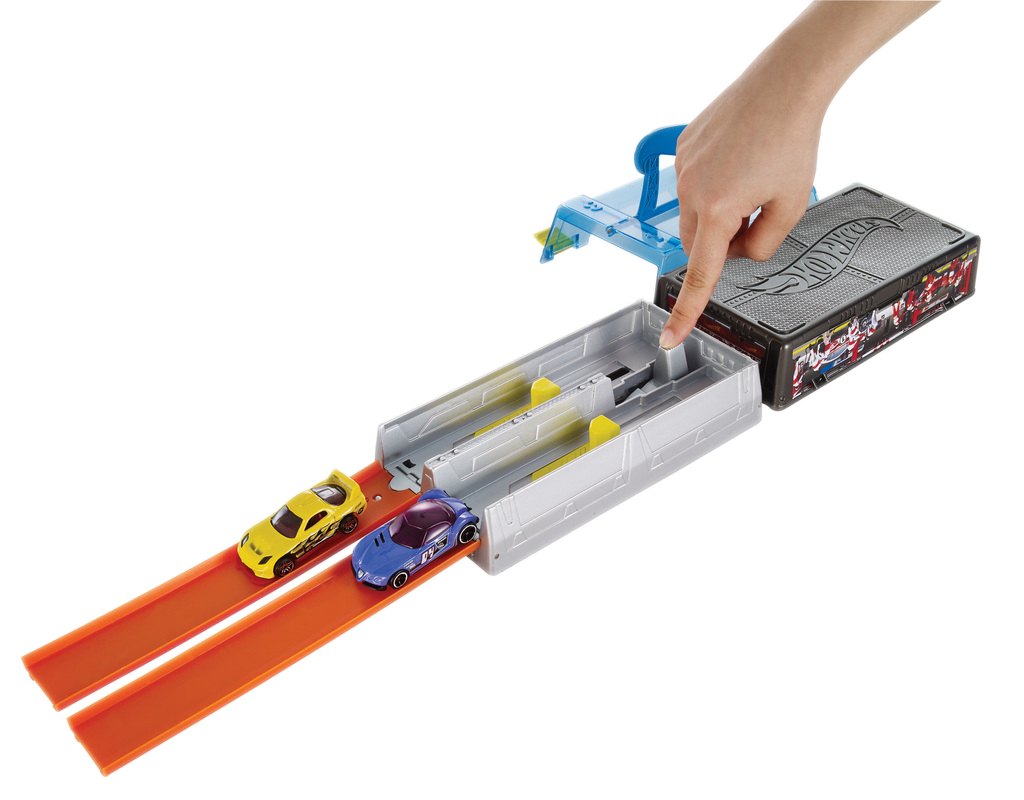
\includegraphics{act2.1.3c-toycarlauncher}	
\end{center}
	
	We want to ask some questions and make some predictions about different cars as they come out of the launcher.  Upon close examination of this launcher, it is noted that the spring is always compressed the same amount each time a car is loaded into the launcher. The spring stays put inside the launcher as the car is pushed out.

	\bitem{What we want to know or predict}
	
	\begin{itemize}
		\item Do all cars come out of the launcher with the same speed?  
		\item If they don't all have the same speed when they come out, what parameters cause the difference?
		\item What do we need to do to get our car to have a higher speed than our friend's cars?
	\end{itemize}
	
	\bitem{Create a Particular Model and Use it to answer the questions}

	Plan what you need to do in your group and how you will proceed BEFORE you start writing on the board.  Be systematic.  Then put your response on the board.	

	\bitem{Suggestions:}
	
	\begin{itemize}
		\item Use the \EnergyInteractionModel{} and the \SOModel{}.
		\item Consider what energy systems are involved.
		\item \textbf{Note:} The car is in contact with the spring while it is compressed and separates from the spring just as the spring reaches its equilibrium length. During the time that the car and spring are together, they behave as a spring-mass system.
		\item To simplify the notation, use ``$d$'' for the distance the spring is compressed instead of ``$\Delta x$''.
	\end{itemize}
	
	\bitem{Be prepared to present a precise, logical, explanation that ``gets at'' the answers to the questions.}
\end{benumerate}

\WCD